\documentclass[11pt,a4paper,openright,twoside]{article}
\usepackage[english]{babel}
\usepackage{newlfont}
\usepackage{color}
\textwidth=450pt\oddsidemargin=0pt
\usepackage{graphicx}
\usepackage{float}
\usepackage{textcomp}
\usepackage{caption}
\usepackage{wrapfig}
\usepackage{subfig}
\usepackage{sidecap}
\usepackage[rlft]{floatflt}
\usepackage{amsmath}
\usepackage{amssymb}
\usepackage{bm}
\usepackage{fancyhdr}
\usepackage{multirow}
\usepackage[utf8x]{inputenc}
\usepackage{fullpage}
\usepackage[Lenny]{fncychap}
\usepackage[T1]{fontenc}
\usepackage[normalem]{ulem}
\usepackage{booktabs}
\usepackage{enumerate}

\usepackage[usenames,dvipsnames]{xcolor}
\usepackage{listings}
\usepackage{xcolor}

\newcommand{\forceindent}{\leavevmode{\parindent=1em\indent}}

\definecolor{light-gray}{gray}{0.95}
\lstset{language=R,
    basicstyle=\small\ttfamily,
    stringstyle=\itshape\color{RedViolet},
    showstringspaces=false,
    %otherkeywords={0,1,2,3,4,5,6,7,8,9},
    morekeywords={TRUE,FALSE, ggplot, data.frame, theme, ylab, xlab},
    deletekeywords={data, frame, beta, c, par, colours, contour, scale,
                    panel, grid, hat},
    keywordstyle=\color{black},%\color{RoyalBlue},
    commentstyle=\itshape\color{PineGreen},
    backgroundcolor=\color{light-gray}
}

\title{CTGT Shortcut - Permutations}
\author{Anna Vesely}
\date{November 2019}





\begin{document}

\maketitle


%\vspace{15mm}



\section{Introduction and Notation}
\paragraph{Permutation test with centered statistics.}
Let $F=\{1,\ldots, f\}$ be the full model, while $S\subseteq F$ is the subset under test by closed testing: $H_S$ is rejected if and only if $H_V$ is rejected for all $V$ such that $S\subseteq V\subseteq F$.

Assume that $T_i$ is the \textbf{standardized} test statistic for the univariate hypothesis $H_i$ and that, for each $V\subseteq F$, the test statistic for $H_V$ can be written as the sum
\[T_V=\sum_{i\in V}T_i.\]
Given a set $\mathcal{P}$ of random permutations (including the identity $\pi_1=$ id) with $|\mathcal{P}|=B$, consider the matrix
\begin{align*}
T=
\begin{pmatrix}
T_1 & \ldots & T_f\\
T_1^2 & \ldots & T_f^2\\
\vdots &  & \vdots\\
T_1^B & \ldots & T_f^B
\end{pmatrix}
\end{align*}
Assume, for simplicity, that the columns are already sorted so that $T_1\geq\ldots\geq T_f$. Subsequently, define the centered test statistics
\begin{align*}
D_i^{\pi}=T_i^{\pi}-T_i,
\end{align*}
so that the observed values are all $D_i=0$, and the variability due to $T_i$ is excluded. The p-value corresponding to $H_V$ is
\begin{align*}
\text{p-value}(V)=\frac{\#\{\pi\,:\,T_V^{\pi}\geq T_V\}}{B}=\frac{\#\{\pi\,:\,D_V^{\pi}\geq 0\}}{B}.
\end{align*}


\vspace{3mm}
\paragraph{Test for a fixed superset size.} Let $m=f-s$ be the number of indices in $F\setminus S$. If $V$ is a superset of $S$, then its size is $|V|=s+v$, with $v\in\{0,1,\ldots,m\}$.

Fix a value $v\in\{0,1,\ldots,m\}$, and consider the set
\[\mathcal{V}_v=\{V\,:\,S\subseteq V\subseteq F,\;|V|=s+v\},\]
as well as
\begin{align*}
&D_S =
\begin{pmatrix}
0\\
D_S^2\\
\vdots\\
D_S^B
\end{pmatrix}
&D_{c} =
\begin{pmatrix}
0 & \ldots & 0\\
D_{c,1}^{2} & \ldots & D_{c,m}^{2}\\
\vdots &  & \vdots\\
D_{c,1}^{B} & \ldots & D_{c,m}^{B}
\end{pmatrix}
\end{align*}
where $D_{c}$ is the matrix of the $m$ individual statistics $D_j^{\pi}$ corresponding to the indices $j\notin S$, sorted in decreasing order within each row: 
\[D_{c,1}^{\pi}\geq\ldots\geq D_{c,m}^{\pi}\quad\forall\,\pi\in\mathcal{P}.\]

The lower and upper bounds for the distribution of $D_V^{\pi}$ are given by the sum of $D_S^{\pi}$ and the $v$ smaller and higher remaining test statistics:
\begin{align*}
& D_{L(v)}^{\pi}=D_S^{\pi}+\sum_{j=m-v+1}^{m} D_{c,j}^{\pi} & D_{U(v)}^{\pi}=D_S^{\pi}+\sum_{j=1}^{v} D_{c,j}^{\pi}.
\end{align*}

Let $c_{L(v)}$ and $c_{U(v)}$ be the ($1-\alpha$)-quantiles of the distribution of the bounds $D_{L(v)}^{\pi}$ and $D_{U(v)}^{\pi}$. The bounds for the fixed size $v$ may be checked in the following way:
\begin{itemize}
\item if $0=D_V\leq c_{L(v)}$, then $H_S$ is not rejected;
\item if $0=D_V > c_{U(v)}$, then $H_V$ is rejected for all $V\in\mathcal{V}_v$, and a different size can be checked;
\item otherwise, the output is indecisive.
\end{itemize}

\begin{figure}[h!]
\centering
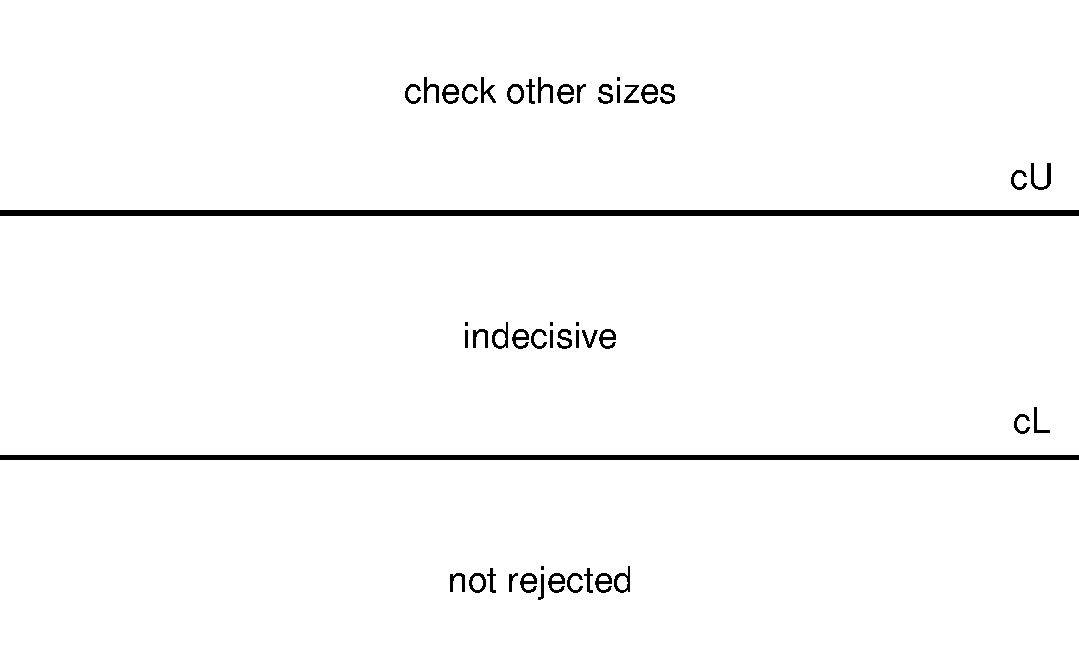
\includegraphics[scale=0.5]{test_areas.pdf}
\label{test_areas}
\caption{Outcomes of the bounds check according to different positions of the point $D_V=0$.}
\end{figure}

\vspace{3mm}
\paragraph{Test.} All the possible superset sizes $v=0,1,\ldots,m$ are checked with the above-mentioned procedure:
\begin{itemize}
\item whenever a size $v^*$ leading to a non-rejection ($c_{L(v^*)}\geq 0$) is found, the algorithm stops and $H_S$ is not rejected;
\item if all sizes $v$ are such that the corresponding hypotheses are rejected with certainty ($c_{U(v)}<0$), $H_S$ is rejected;
\item otherwise, the sizes $v$ leading to an indecisive output ($c_{L(v)}<0\leq c_{U(v)}$) are examined with a step-by-step method.
\end{itemize}

The analysis starts with the extremes $v=0$ and $v=m$, corresponding to $S$ and $F$. In both cases the output cannot be indecisive, as the lower and upper bounds coincide: $c_{L(0)}=c_{U(0)}=c_0$ and $c_{L(m)}=c_{U(m)}=c_m$. If neither case leads to a non-rejection, the other sizes are checked in
\begin{itemize}
\item increasing order ($v=1,\ldots,m-1$) if $c_{m}\leq c_{0}<0$;
\item decreasing order ($v=m-1,\ldots,1$) if $c_{0}< c_{m}<0$.
\end{itemize}
Indeed, in the first case the rejection for $S$ is less extreme than that for $F$; hence we expect that an eventual non-rejection will be likely found with small sizes, when adding one or more indices to $S$. On the contrary, in the second case we expect that an eventual non-rejection will be likely found when removing one or more indices from $F$.

\vspace{3mm}
\paragraph{Step-by-step method.} Let $i_1$ be the index of the highest observed statistic in $F\setminus S$,
\[T_{i_1}=\max\{T_j\,;\,j\in F\setminus S\},\]
corresponding to the centered statistic $D_{c,1}$. Similarly, let $i_n$ be the index of the $n$-th highest observed statistic, corresponding to $D_{c,n}$.

For each size $v$ leading to an indecisive outcome, the set $\mathcal{V}_v$ is partitioned in
\begin{itemize}
\item $\mathcal{V}_v(-i_1)=\{V\in\mathcal{V}\,:\,i_1\notin V\}=\{V\,:\,S\subseteq V\subseteq F\setminus\{i_1\},\;|V|=v+s\}$
\item $\mathcal{V}_v(+i_1)=\{V\in\mathcal{V}\,:\,i_1\in V\}=\{V\,:\,S\cup\{i_1\}\subseteq V\subseteq F,\;|V|=v+s\}$.
\end{itemize}
We expect that the quantities $D_{i_1}^{\pi}=T_{i_1}^{\pi}-T_{i_1}$ will likely be small, and thus in the analysis of $(-i_1)$ the lower bound will likely increase. In both cases, however, the bounds will never become wider.

The step-by-step method is a depth-first search. First, it explores the cases $(-i_1)$ and $(+i_1)$, and enumerates the eventual indecisive sizes. If a non-rejection is found, it stops and $H_S$ is not rejected. Otherwise it further divides the first case into $(-i_1,-i_2)$ and $(-i_1,+i_2)$. Such procedure is iterated until $(-i_1,\ldots,-i_h)$ produces no indecisive sizes; then the algorithm analyzes $(-i_1,\ldots,-i_{h-1},+i_h)$.

The cases to be examined are stacked in a last-in-first-out pile. At each step, the first element is removed, and the two elements derived as subcases, if non-null, are added to the list:
\begin{align*}
\begin{matrix}
\text{step 1} & (-i_1) & (+i_1) &  &  & \\
\text{step 2} & (-i_1,-i_2) & (-i_1,+i_2) & (+i_1) &  \\
\text{step 3}  &(-i_1,-i_2,-i_3) & (-i_1,-i_2,+i_3) & (-i_1,+i_2) & (+i_1) \\
\ldots &  &  &  &  
\end{matrix}
\end{align*}

Each element of the list is characterized by
\begin{itemize}
\item $n$, the total number of test statistics that have been considered (removed or kept);
\item $D_{\text{fixed}}$, the sum of $D_S$ and the test statistics that have been kept;
\item $ind.free$, the vector of the indecisive sizes minus the number of kept statistics.
\end{itemize}

When an element is divided into subcases, the statistics corresponding to indices $i_1,\ldots,i_{n}$ are removed from $D_c$ to define $D_{c\text{(new)}}$. Moreover, $D_{\text{fixed(new)}}^{\pi}$ is defined as the sum of $D_{\text{fixed}}$ and the $n$-th highest test statistic in $F\setminus S$. If $R$ and $K$ denote the distributions when such statistic is removed and kept, respectively, then
\begin{align*}
&R_{L(v)}^{\pi}=D_{\text{fixed}}^{\pi}+D_{c\text{(new)},m-v+1}^{\pi} + A_{L(v)}^{\pi} & K_{L(v)}^{\pi}=D_{\text{fixed(new)}}^{\pi}+A_{L(v)}^{\pi}\\
&R_{U(v)}^{\pi}=D_{\text{fixed}}^{\pi}+D_{c\text{(new)},v}^{\pi}+A_{U(v)}^{\pi} & K_{U(v)}^{\pi}=D_{\text{fixed(new)}}^{\pi}+A_{U(v)}^{\pi}
\end{align*}
where
\begin{align*}
& A_{L(v)}^{\pi}=\sum_{j=m-v+2}^{m} D_{c\text{(new)},j}^{\pi} & A_{U(v)}^{\pi}=\sum_{j=1}^{v-1}  D_{c\text{(new)},j}^{\pi}.
\end{align*}

\begin{lstlisting}
incr.bab.set <- function(Dfixed, Dfixed.new){
	z <<- 1 # previous size

	# bounds when removing (R) or keeping (K)
	Rlow <<- Dfixed
	Rup <<- Rlow
	Klow <<- Dfixed.new
	Kup <<- Klow
}
\end{lstlisting}


\begin{lstlisting}
decr.bab.set <- function(Dfixed, Dfixed.new, m, Dc.new){
	z <<- m
	Dtot <<- rowSums(Dc.new)

	# bounds when removing (R) or keeping (K)
	Rlow <- Dfixed + Dtot
	Rup <- Rlow
	Klow <- Dfixed.new + Dtot
	Kup <- Klow
}
\end{lstlisting}

\begin{lstlisting}
incr.bab.loop <- function(z, v, ind.free, Dc.new, m, B){
	cond <- (v-1 < z)
	Alow <- IFELSE(cond, rep(0,B),
	   rowSums(Dc.new[,((m-v+2):(m-z+1)])
	Rlow <<- Rlow + Dc.new[,m-v+1] + Alow
	IF NOT(above.quantile(Rlow), alpha){
		NOT REJECTED
	}

	Klow <<- Klow + Alow
	IF NOT(above.quantile(Klow), alpha){
		NOT REJECTED
	}

	Aup <- IFELSE(cond, rep(0,B),
	   rowSums(Dc.new[,(z):(v-1)])
	Rup <<- Rup + Dc.new[,v] + Aup
	IF NOT(above.quantile(Rup), alpha){
		ind.remove <<- c(ind.remove, ind.free[i])
	}

	Kup <<- Kup + Aup
	IF NOT(above.quantile(Kup), alpha){
		ind.keep <<- c(ind.keep, ind.free[i])
	}
}
\end{lstlisting}

\begin{lstlisting}
decr.bab.loop <- function(z, v, ind.free, Dc.new, m, B){
	cond <- (v+1 > z)
	Alow <- IFELSE(cond, rep(0,B),
	   rowSums(Dc.new[,((m-z+1):(m-v)])
	Rlow <<- Rlow - Alow
	IF NOT(above.quantile(Rlow), alpha){
		NOT REJECTED
	}

	Klow <<- Klow - Dc.new[,m-v+1] - Alow 
	IF NOT(above.quantile(Klow), alpha){
		NOT REJECTED
	}

	Aup <- IFELSE(cond, rep(0,B),
	   rowSums(Dc.new[,(v+1):z])
	Rup <<- Rup - Aup
	IF NOT(above.quantile(Rup)){
		ind.remove <<- c(ind.remove, ind.free[i])
	}

	Kup <<- Kup - Dc.new[,v] - Aup
	IF NOT(above.quantile(Kup), alpha){
		ind.keep <<- c(ind.keep, ind.free[i])
	}
}
\end{lstlisting}


\begin{lstlisting}
# tolgo il primo della pila e creo i nodi figli
# se questi non sono vuoti
# li aggiungo in cima alla lista
# (per primo quello remove)
# itero finche non si svuota oppure trovo
# un non-reject

children.nodes <- function(n, Dfixed, ind.free, Dc, compl.indices){
	# the first n highest statistics are removed from Dc
	Dc.new <- Dc[-el. corresponding to indices in
	   compl.indices[1:n] in I]
	Dfixed.new <- Dfixed + Dc[el. corresponding to index
	   compl.indices[n] in I]

	L <- length(ind.free)
	i <- 1
	v <- ind.free[1] # first size	
	ind.remove <<- c() # indecisive free sizes after removing
	ind.keep <<- c() # indecisive free sizes after keeping

	IFELSE(incr.order, incr.bab.set(Dfixed, Dfixed.new),
	   decr.bab.set(Dfixed, Dfixed.new, m, Dc.new))

	WHILE (i <= L){
		IFELSE(incr.order, incr.bab.loop(z, v, ind.free, Dc.new, m, B),
		   decr.bab.loop(z, v, ind.free, Dc.new, m, B))

		z <- v
		i <- i+1
		v <- indecisive[i]
	}

	RETURN
		# n+1, Dfixed, ind.remove
		#n+1, Dfixed.new, ind.keep
# vanno aggiunti alla pila se non sono vuoti
}




# sistemare i return delle funzioni
# dentro incr.bab.loop
# e nella funzione principale
#(si stoppa se non-reject)
\end{lstlisting}
















\newpage
\section{Algorithm}
The algorithm requires
\begin{itemize}
\item a $B\times f$ matrix $T$ where the columns correspond to individual hypotheses and are not necessarily ordered, while the rows correspond to random permutations (with $\pi_1=$ id);
\item a subset $S$ of indices under test;
\item a significance level $\alpha$ (by default 0.05).
\end{itemize}


% ------------------------------------------------------------------------------------%

\vspace{3mm}
\paragraph{Main Functions}
The function \texttt{perm.setting} sorts the columns of $T$ in increasing order, and then defines the matrix $D$ of centered test statistics, sorted within each row. Another matrix $I$ keeps track of the original indices: if $D_j^\pi$ corresponds to the individual test statistic on index $i$ in the input matrix, then $I_{\pi j}=i$. This first step will be kept apart from the following functin, so that the matrices $D$ and $I$ can be defined only once even when different subsets $S$ are checked.
\begin{lstlisting}
perm.setting <- function(T){
	IF NOT(check.matrix(T)){
		STOP with error message
	}
	
	i.vec <- (1,...,f)
	T <- T[columns sorted so that T[1,] is in incr. order]
	i.vec <- i.vec[reordered as T[1,]]
	# note: the columns can be sorted with other criteria

	I <- matrix(B rows, each equal to i.vec)
	D <- T[each column is centered with respect to its first el.]
	D <- D[are sorted in incr. order within each row
	   except the first]
	I <- I[reordered as D]
	# B times f matrices

	RETURN list("D"=D, "I"=I)
}
\end{lstlisting}


% ------------------------------------------------------------------------------------%


\vspace{3mm}
The function \texttt{perm.test} checks the null hypothesis on the set of indices $S$. The inner functions are displayed in the following section.

\textbf{Check the link in the comment. Now I need to implement the tree structure and the BAB.}
% https://www.geeksforgeeks.org/inorder-tree-traversal-without-recursion/




\begin{lstlisting}
perm.test(D, I, S, alpha){
	IF NOT(check.matrix(D) AND check.matrix(I)){
		STOP with error message
	}
	B <- nrow(D)
	f <- ncol(D)

	IF NOT(check.indices(I, B, f)){
		STOP with error message
	}

	IF NOT(check.hp(S, f)){
		STOP with error message
	}
	S <- unique(S)
	s <- length(S)
	m <- f-s

	IF NOT(0 < alpha < 1){
		STOP with error message
	}

	# if m=0 (s=f), we are testing all the indices
	IF (m == 0){
		rej <- above.quantile(rowSums(D), alpha)
		RETURN list("rejected"=rej, "bab.steps"=0)
	}


	Ds <- D[elements corresponding in I to indices in S]
	# D_j^pi is removed if I[pi,j] is in S
	Ds <- rowSums(Ds) # vector of length B
	
	Dfull <- rowSums(D)
	# sum of all test statistics

	# v=0 and v=m
	extremes <- extremes.check(Ds, Dfull, alpha)
	IF NOT(extremes){
		RETURN list("rejected"=FALSE, "bab.steps"=0)
	}

	compl.indices <- I[1,][- indices in S]
	# indices not in S in order
	Dc <- D[-elements corresponding in I to indices in S]
	# B times m matrix

	middle <- IFELSE(incr.order, incr.check(Ds, Dc, m, alpha),
	   decr.check(Dfull, Dc, m, alpha))
	IF NOT(middle){
		RETURN list("rejected"=FALSE, "bab.steps"=0)
	}

%%%

	
	# STEP-BY-STEP METHOD

	n <- 1
	A <- c()
	list.of.ind <- list(list("sel"=c(), "indecisive"=indecisive))

	WHILE (length(list.of.ind) > 0){
		A <- cbind(A, D[el. corresponding to index (m-n) in I])
		D <- D[- el. corresponding to index (m-n) in I]
		I <- D[- el. equal to (m-n)]
		
		temp <- list.of.ind
		
		FOR (e IN list.of.ind){
			# function defined in the following paragraph:
			bab <- bab.step(n, e$sel, e$indecisive)
			IF (bab$not.rejected){
				RETURN list("out"="not rejected",
				   "bab.steps"=n)
			}
		}

		list.of.ind <- temp
		n <- n+1
	}

	# if the list of indecisive sizes for all branches is null:
	RETURN list("out"="rejected", "bab.steps"=n-1)
}
\end{lstlisting}


% ------------------------------------------------------------------------------------%

\vspace{3mm}
\paragraph{Internal Functions}
The following functions are used to check the inputs and some conditions.
\begin{lstlisting}
# TRUE if an object M is a matrix of finite numbers
check.matrix <- function(M){
	out <- (M is a matrix of finite numbers)
	RETURN out
}
\end{lstlisting}

\begin{lstlisting}
# TRUE if a matrix M is a well-defined matrix of indices
# with given dimensions
check.indices <- function(M, n.row, n.col){
	out <- (nrow(I) == n.row AND ncol(I) == n.col AND
	   each row of I contains the integers from 1 to n.col)
	RETURN out
}
\end{lstlisting}

\begin{lstlisting}
# TRUE if an object X is a vector of integers
# between 1 and a given maximum
check.hp <- function(X, n.max){
	out <- (X is a numerical vector AND
	   its elements are integers between 1 and n.max)
}
\end{lstlisting}

\begin{lstlisting}
# TRUE if zero is greater than the sample quantile of a vector X
above.quantile <- function(X, alpha){
	c <- quantile(X, (1-alpha))
	out <- (sign(c) == -1) # 0 > c
	RETURN out
}
\end{lstlisting}


% ------------------------------------------------------------------------------------%


\vspace{3mm}
The following functions check different superset sizes. In particular, \texttt{incr.check} and \texttt{decr.check} exploit the fact that
\begin{align*}
&D_{L(v)}=D_{L(v-1)}+D_{m-v+1} & D_{U(v)}=D_{U(v-1)}+D_{v}\\
&D_{L(v)}=D_{L(v+1)}-D_{m-v} & D_{U(v)}=D_{U(v+1)}-D_{v+1}.
\end{align*}

\begin{lstlisting}
# check of the cases v=0 and v=m
# FALSE in case of a non-rejection, TRUE otherwise
# it creates incr.order, TRUE if the order to be used for the middle
# sizes is increasing
extremes.check <- function(Ds, Dfull, alpha)
	# v=0
	c0 <- quantile(Ds, (1-alpha))
	# stop (not rejected) if 0 <= c0
	IF (sign(c0) > -1){
		RETURN FALSE
	}

	# v=m
	cfull <- quantile(Dfull, (1-alpha))
	# stop (not rejected) if 0 <= cfull
	IF (sign(cfull) > -1){
		RETURN FALSE
	}

	# if cfull <= c0, sizes will be explored in incr. order
	incr.order <<- IFELSE (cfull <= c0, TRUE, FALSE)
	RETURN TRUE
}\end{lstlisting}

\begin{lstlisting}
# check of sizes v=1,...,m-1
# in increasing order
# FALSE in case of a non-rejection, TRUE otherwise
# it creates the vector of indecisive sizes
incr.check <- function(Ds, Dc, m, alpha){
	v <- 1
	Dlow <- Ds
	Dup <- Ds
	indecisive <<- c() # keeps track of indecisive sizes

	WHILE (v < m){
		Dlow <- Dlow + Dc[,m-v+1]
		# stop (not rejected) if 0 <= clow
		IF NOT(above.quantile(Dlow), alpha){
			RETURN FALSE
		}

		Dup <- Dup + Dc[,v]
		# indecisive if if clow < 0 <= cup
		IF NOT(above.quantile(Dup), alpha){
			indecisive <<- c(indecisive, v)
		}
	
		v <- v+1
	}
	RETURN TRUE
}
\end{lstlisting}

\begin{lstlisting}
# check of sizes v=m-1,...,1
# in decreasing order
# FALSE in case of a non-rejection, TRUE otherwise
# it creates the vector of indecisive sizes
decr.check <- function(Dfull, Dc, m, alpha){
	v <- m-1
	Dlow <- Dfull
	Dup <- Dfull
	indecisive <<- c() # keeps track of indecisive sizes

	WHILE (v > 0){
		Dlow <- Dlow - Dc[,m-v]
		# stop (not rejected) if 0 <= clow
		IF NOT(above.quantile(Dlow)){
			RETURN FALSE
		}

		Dup <- Dup - Dc[,v+1]
		# indecisive if if clow < 0 <= cup
		IF NOT(above.quantile(Dup)){
			indecisive <<- c(indecisive, v)
		}
	
		v <- v-1
	}
	RETURN TRUE
}
\end{lstlisting}



\newpage
\section{Pseudo Code}
The algorithm requires:
\begin{itemize}
\item the matrix $T$ having in each row the individual test statistics corresponding to a permutation (the first row corresponds to the identity)
\begin{align*}
T=
\begin{pmatrix}
T_1 & \ldots & T_f\\
T_1^2 & \ldots & T_f^2\\
\vdots &  & \vdots\\
T_1^B & \ldots & T_f^B
\end{pmatrix}
\end{align*}
\item a subset $S$ of indices under test;
\item a significance level $\alpha$ (by default 0.05).
\end{itemize}

\vspace{3mm}
\noindent
$T$ is checked and the matrix $D$ of centered statistics is defined. The first row of $D$ is deleted, since it is always null (but the value 0 will be added again when computing the sample quantiles). This function will be kept separated, so that the matrix $D$ can be defined only once even when different subsets $S$ are checked.
\begin{lstlisting}
perm.setting <- function(T){
	IF NOT(T is a matrix of finite numbers){
		STOP with error message
	}

	D <- T[columns sorted so that T[1,] is in incr. order]
	# note: the columns can be sorted with other criteria
	D <- D[each column is centered with respect to its first el.]
	D <- D[-1,] # as the first column is null
	RETURN D
}


# function that returns TRUE if zero is smaller than
# the sample quantile of a vector c(0,X)
under.quantile <- function(X, alpha){
	c <- quantile(c(0,X), (1-alpha))
	out <- (0 <= c)
	RETURN out
}
\end{lstlisting}

\vspace{3mm}
\noindent
$S$ and $\alpha$ are checked. Then
\begin{align*}
&Ds =
\begin{pmatrix}
D_S^2\\
\vdots\\
D_S^B
\end{pmatrix}
&D =
\begin{pmatrix}
D_{S^c,\,(1)}^{2} & \ldots & D_{S^c,\,(m)}^{2}\\
\vdots &  & \vdots\\
D_{S^c,\,(1)}^{B} & \ldots & D_{S^c,\,(m)}^{B}
\end{pmatrix}
\end{align*}
where $m=f-s$. The matrix $I$ keeps track of the indices of $D$ before the reordering:
\[I_{\pi j}=i\quad\Longleftrightarrow\quad D_{S^c,\,(j)}^{\pi}=D_{S^c,\,i}^{\pi}.\]

Let $z=v-s\in\{0,\ldots,m\}$. Both for $z=0$ and $z=m$ (i.e. $v=s$ and $v=f$),
\[D_{L(v)}^{\pi}=D_{U(v)}^{\pi}=D_V^{\pi}.\]
The check on different $z$ starts with $z=0$; in the particular case of $m=0$ (i.e. $s=f$), the algorithm stops.

For the following values of $z$, the lower and upper bounds are updated by adding the elements of columns $z$ and $m-z+1$, respectively:
\begin{align*}
& D_{L(v)}=Ds+\sum_{j=1}^{z} D_j & D_{U(v)}=Ds+\sum_{j=m-z+1}^{m} D_j\\
& D_{L(v+1)}=D_{L(v)}+D_{z+1} & D_{U(v+1)}=D_{U(v)}+D_{m-(z+1)+1}.
\end{align*}
The vector $indecisive$ keeps track of the sizes to be checked later with the step-by-step method, if needed. If there are no indecisive values, the null hypothesis is rejected.
\begin{lstlisting}
# D is the matrix of centered test statistics
perm.check(S, D, alpha){
	IF NOT(0 < alpha < 1){
		STOP with error message
	}

	IF NOT(S is a numerical vector){
		STOP with error message
	}
	
	B <- nrow(D)
	f <- ncol(D)
	S <- unique(S)
	s <- length(S)
	m <- f-s

	IF NOT(the el. of S are integers between 1 and f){
		STOP with error message
	}


	# s=f:
	IF (m == 0){
		Ds <- rowSums(D)
	}
	ELSE{
		Ds <- rowSums(D[,S])
		D <- D[,-S]
		I <- matrix((B-1) rows, each equal to 1,...,m)

		D <- D[within each row el. are sorted in incr. order]
		I <- I[reordered as D]
	}


	# z=v-s, from 0 to m
	# first check z=0 (v=s):
	IF (under.quantile(Ds, alpha)){
		RETURN list("out"="not rejected", "bab.steps"=0)
	}

	IF (m == 0){
		RETURN list("out"=not rejected, "bab.steps"=0)
	}


	# then check z=1,...,m-1:
	indecisive <- c()
	z <- 1

	WHILE (z < m){
		Dlow <- Ds + D[,z]
		IF (under.quantile(Dlow, alpha)){
			RETURN list("out"="not rejected",
			   "bab.steps"=0) # break
		}

		Dup <- Ds + D[,m-z+1]
		IF (under.quantile(Dup, alpha)){
			indecisive <- c(indecisive, z)
		}
	
		z <- z+1
	}


	# finally check z=m (v=f):
	# now Dlow = Dup = D
	IF (under.quantile(Dlow, alpha)){
		RETURN list("out"="not rejected", "bab.steps"=0)
	}


	IF (indecisive is null){
		RETURN list("out"="rejected", "bab.steps"=0)
	}

	
	# STEP-BY-STEP METHOD

	n <- 1
	A <- c()
	list.of.ind <- list(list("sel"=c(), "indecisive"=indecisive))

	WHILE (length(list.of.ind) > 0){
		A <- cbind(A, D[el. corresponding to index (m-n) in I])
		D <- D[- el. corresponding to index (m-n) in I]
		I <- D[- el. equal to (m-n)]
		
		temp <- list.of.ind
		
		FOR (e IN list.of.ind){
			# function defined in the following paragraph:
			bab <- bab.step(n, e$sel, e$indecisive)
			IF (bab$not.rejected){
				RETURN list("out"="not rejected",
				   "bab.steps"=n)
			}
		}

		list.of.ind <- temp
		n <- n+1
	}

	# if the list of indecisive sizes for all branches is null:
	RETURN list("out"="rejected", "bab.steps"=n-1)
}
\end{lstlisting}

\vspace{3mm}
\noindent
The step by step method checks the sizes $z\in\{1,\ldots,m-1\}$ that are indecisive. The elements corresponding to the highest statistic $T_{m}$ are separated from $D$ and stored in the vector $A_1$.

Let $R_{L(v)}^{\pi}$ and $R_{U(v)}^{\pi}$ be the bounds for $\mathcal{V}_1$ (when $T_{m}$ is removed), and $K_{L(v)}^{\pi}$ and $K_{U(v)}^{\pi}$ the bounds for $\mathcal{V}_2$ (when $T_{m}$ is kept):
\begin{align*}
& R_{L(v)}^{\pi}=Ds^{\pi}+\sum_{j=1}^{z} D_j^{\pi} & K_{L(v)}^{\pi}=Ds^{\pi}+A_1^{\pi}+\sum_{j=1}^{z-1} D_j^{\pi}=R_{L(v)}^{\pi} - D_z^{\pi} + A_1^{\pi}\\
& R_{U(v)}^{\pi}=Ds^{\pi}+\sum_{j=m-z+1}^{m} D_j^{\pi} & K_{U(v)}^{\pi}=Ds^{\pi}+A_1^{\pi}+\sum_{j=m-z+2}^{m} D_j^{\pi}=R_{U(v)}^{\pi} - D_{m-z+1}^{\pi} + A_1^{\pi}\\
\end{align*}

As long as there are non-null sets of indecisive sizes, such procedure is iterated.

Before step $n$, the columns of a matrix $A$ keep track of the elements that have already been separated from $D$ (those corresponding to $T_{m},\ldots T_{m-n-1}$). There are at most $2^{n-1}$ vectors of indecisive sizes, each corresponding to a subset where only some columns of $A$ (identified by a vector $sel$ of indices) were kept.

At step $n$, the elements corresponding to $T_{m-n}$ are separated from $D$ and stored as the $n$-th column of $A$. For each couple ($indecisive$, $set$), the subsets where $T_{m-n}$ is removed or kept are analyzed:
\begin{align*}
& R_{L(v)}^{\pi}=Ds^{\pi}+\sum_{a\in sel}A_a^{\pi}+\sum_{j=1}^{z-|sel|} D_j^{\pi} & K_{L(v)}^{\pi}=R_{L(v)}^{\pi} - D_z^{\pi} + A_n^{\pi}\\
& R_{U(v)}^{\pi}=Ds^{\pi}+\sum_{a\in sel}A_a^{\pi}+\sum_{j=m-z+1+|sel|}^{m} D_j^{\pi} & K_{U(v)}^{\pi}=R_{U(v)}^{\pi} - D_{m-z+1}^{\pi} + A_n^{\pi}\\
\end{align*}
\begin{lstlisting}
bab.step <- function(n, sel, indecisive){
	ind.remove <- c() # indecisive sizes after removing
	ind.keep <- c() # indecisive sizes after keeping

	z.prev <- 0
	i <- 1
	n.sel <- length(sel)
	z <- indecisive[i] - n.sel

	Rlow <- Ds + rowSums(A[sel])
	Rup <- Rlow

	WHILE (i <= length(indecisive)){
		Rlow <- Rlow + rowSums(D[,((z.prev+1):z)])
		IF (under.quantile(Rlow, alpha)){
			RETURN list("not.rejected"=TRUE,
			   "ind.remove"=c(), "ind.keep"=c())
		}

		Klow <- Rlow + A[n] - D[,z]
		IF (under.quantile(Klow, alpha)){
			RETURN list("not.rejected"=TRUE,
			   "ind.remove"=c(), "ind.keep"=c())
		}

		Rup <- Rup + rowSums(D[,((m-z+1):(m-z.prev)])
		IF (under.quantile(Rup, alpha)){
			ind.remove <- c(ind.remove, indecisive[i])
		}

		Kup <- Rup + A[n] - D[,m-z+1]
		IF (under.quantile(Kup, alpha)){
			ind.keep <- c(ind.keep, indecisive[i])
		}

		z.prev <- z
		i <- i+1
		z <- indecisive[i] - n.sel
	}

	RETURN list("not.rejected"=FALSE, "ind.remove"=ind.remove,
	   "ind.keep"=ind.keep)
}
\end{lstlisting}

A




\end{document}